\section{时间隐通道验证方案设计}
\label{chap:linphone:designation}

本节主要介绍Linphone环境下,时间隐通道的模块设计,及模块之间的关联与数据流。

\subsection{设计架构及模块关联}
\label{chap:linphone:designation:struct}

\insertFigure{
	\begin{figure}
		\centering
        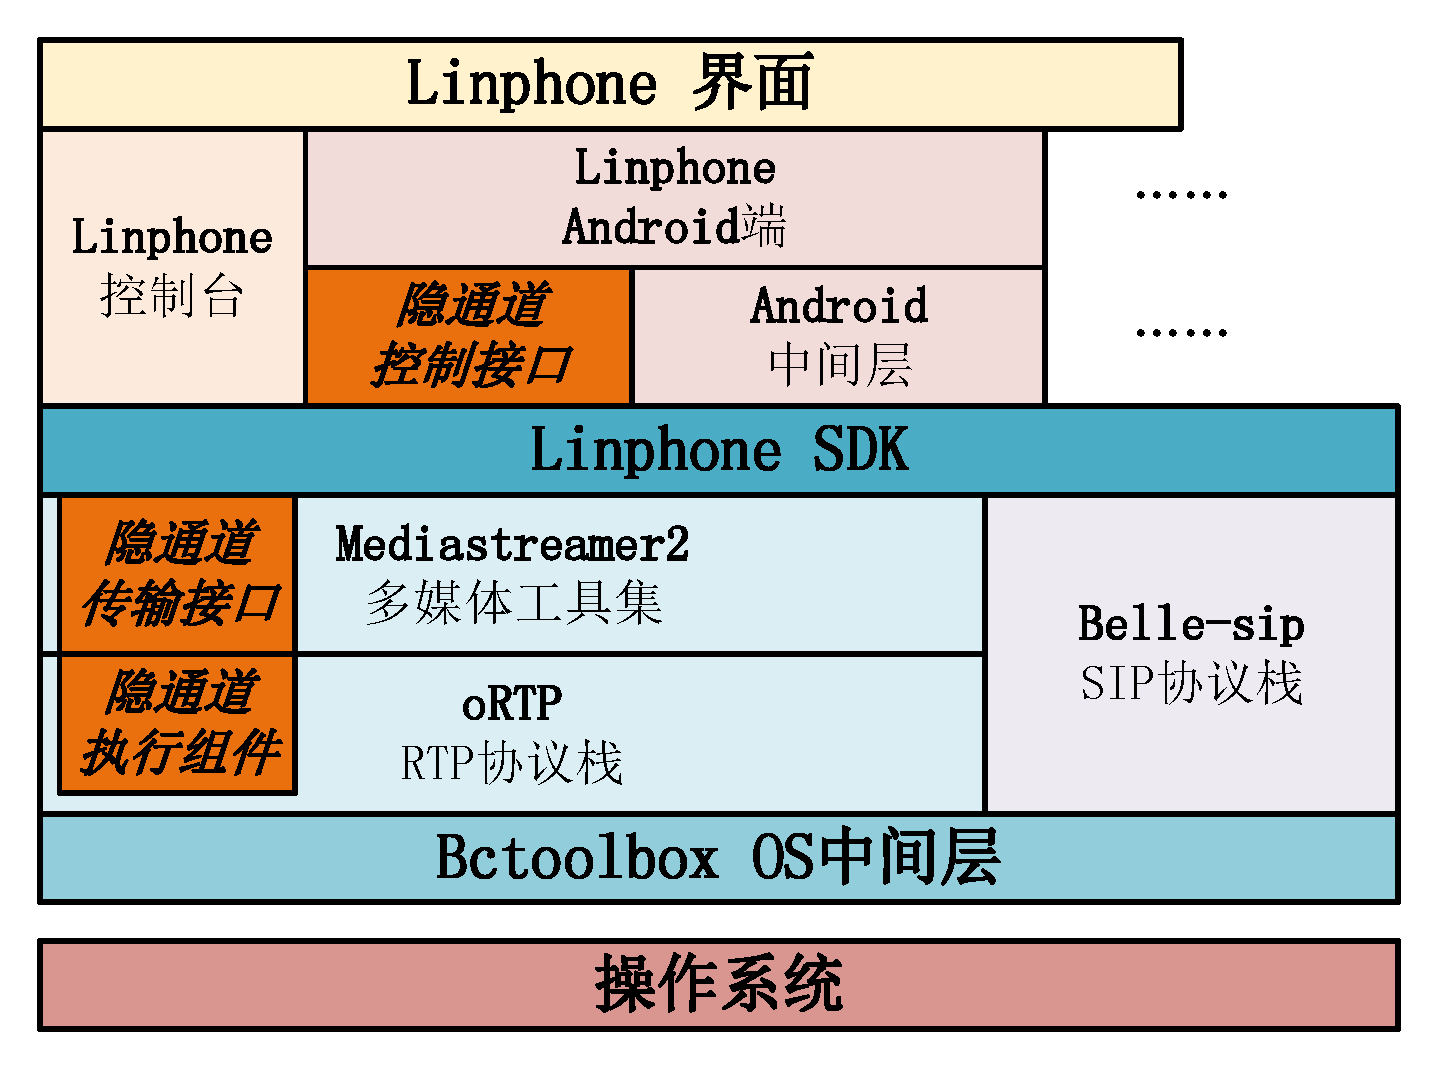
\includegraphics[width=0.7\textwidth]{chapters/chapter6/figures/ctc-struct.pdf}
        \caption{Linphone中时间隐通道模块分布图}
        \label{fig:6:ctc-struct}
    \end{figure}
}

如图\nref{fig:6:ctc-struct},构建时间隐通道添加的模块包括三部分,分别为隐通道控制接口、隐通道传输接口及隐通道执行组件。其中,隐通道控制接口位于Linphone Android端的界面层,负责接收用户的控制命令,并反馈响应结果。隐通道传输接口位于Mediastreamer2层中,负责在Linphone SDK中创建对外接口,并连接执行组件,实现数据及控制流传输。隐通道执行组件位于oRTP层,负责控制与监听RTP数据包传输,以及时间隐通道传输逻辑的实现。

\subsection{用户控制接口设计}
\label{chap:linphone:designation:ui}

\insertFigure{
	\begin{figure}
		\centering
        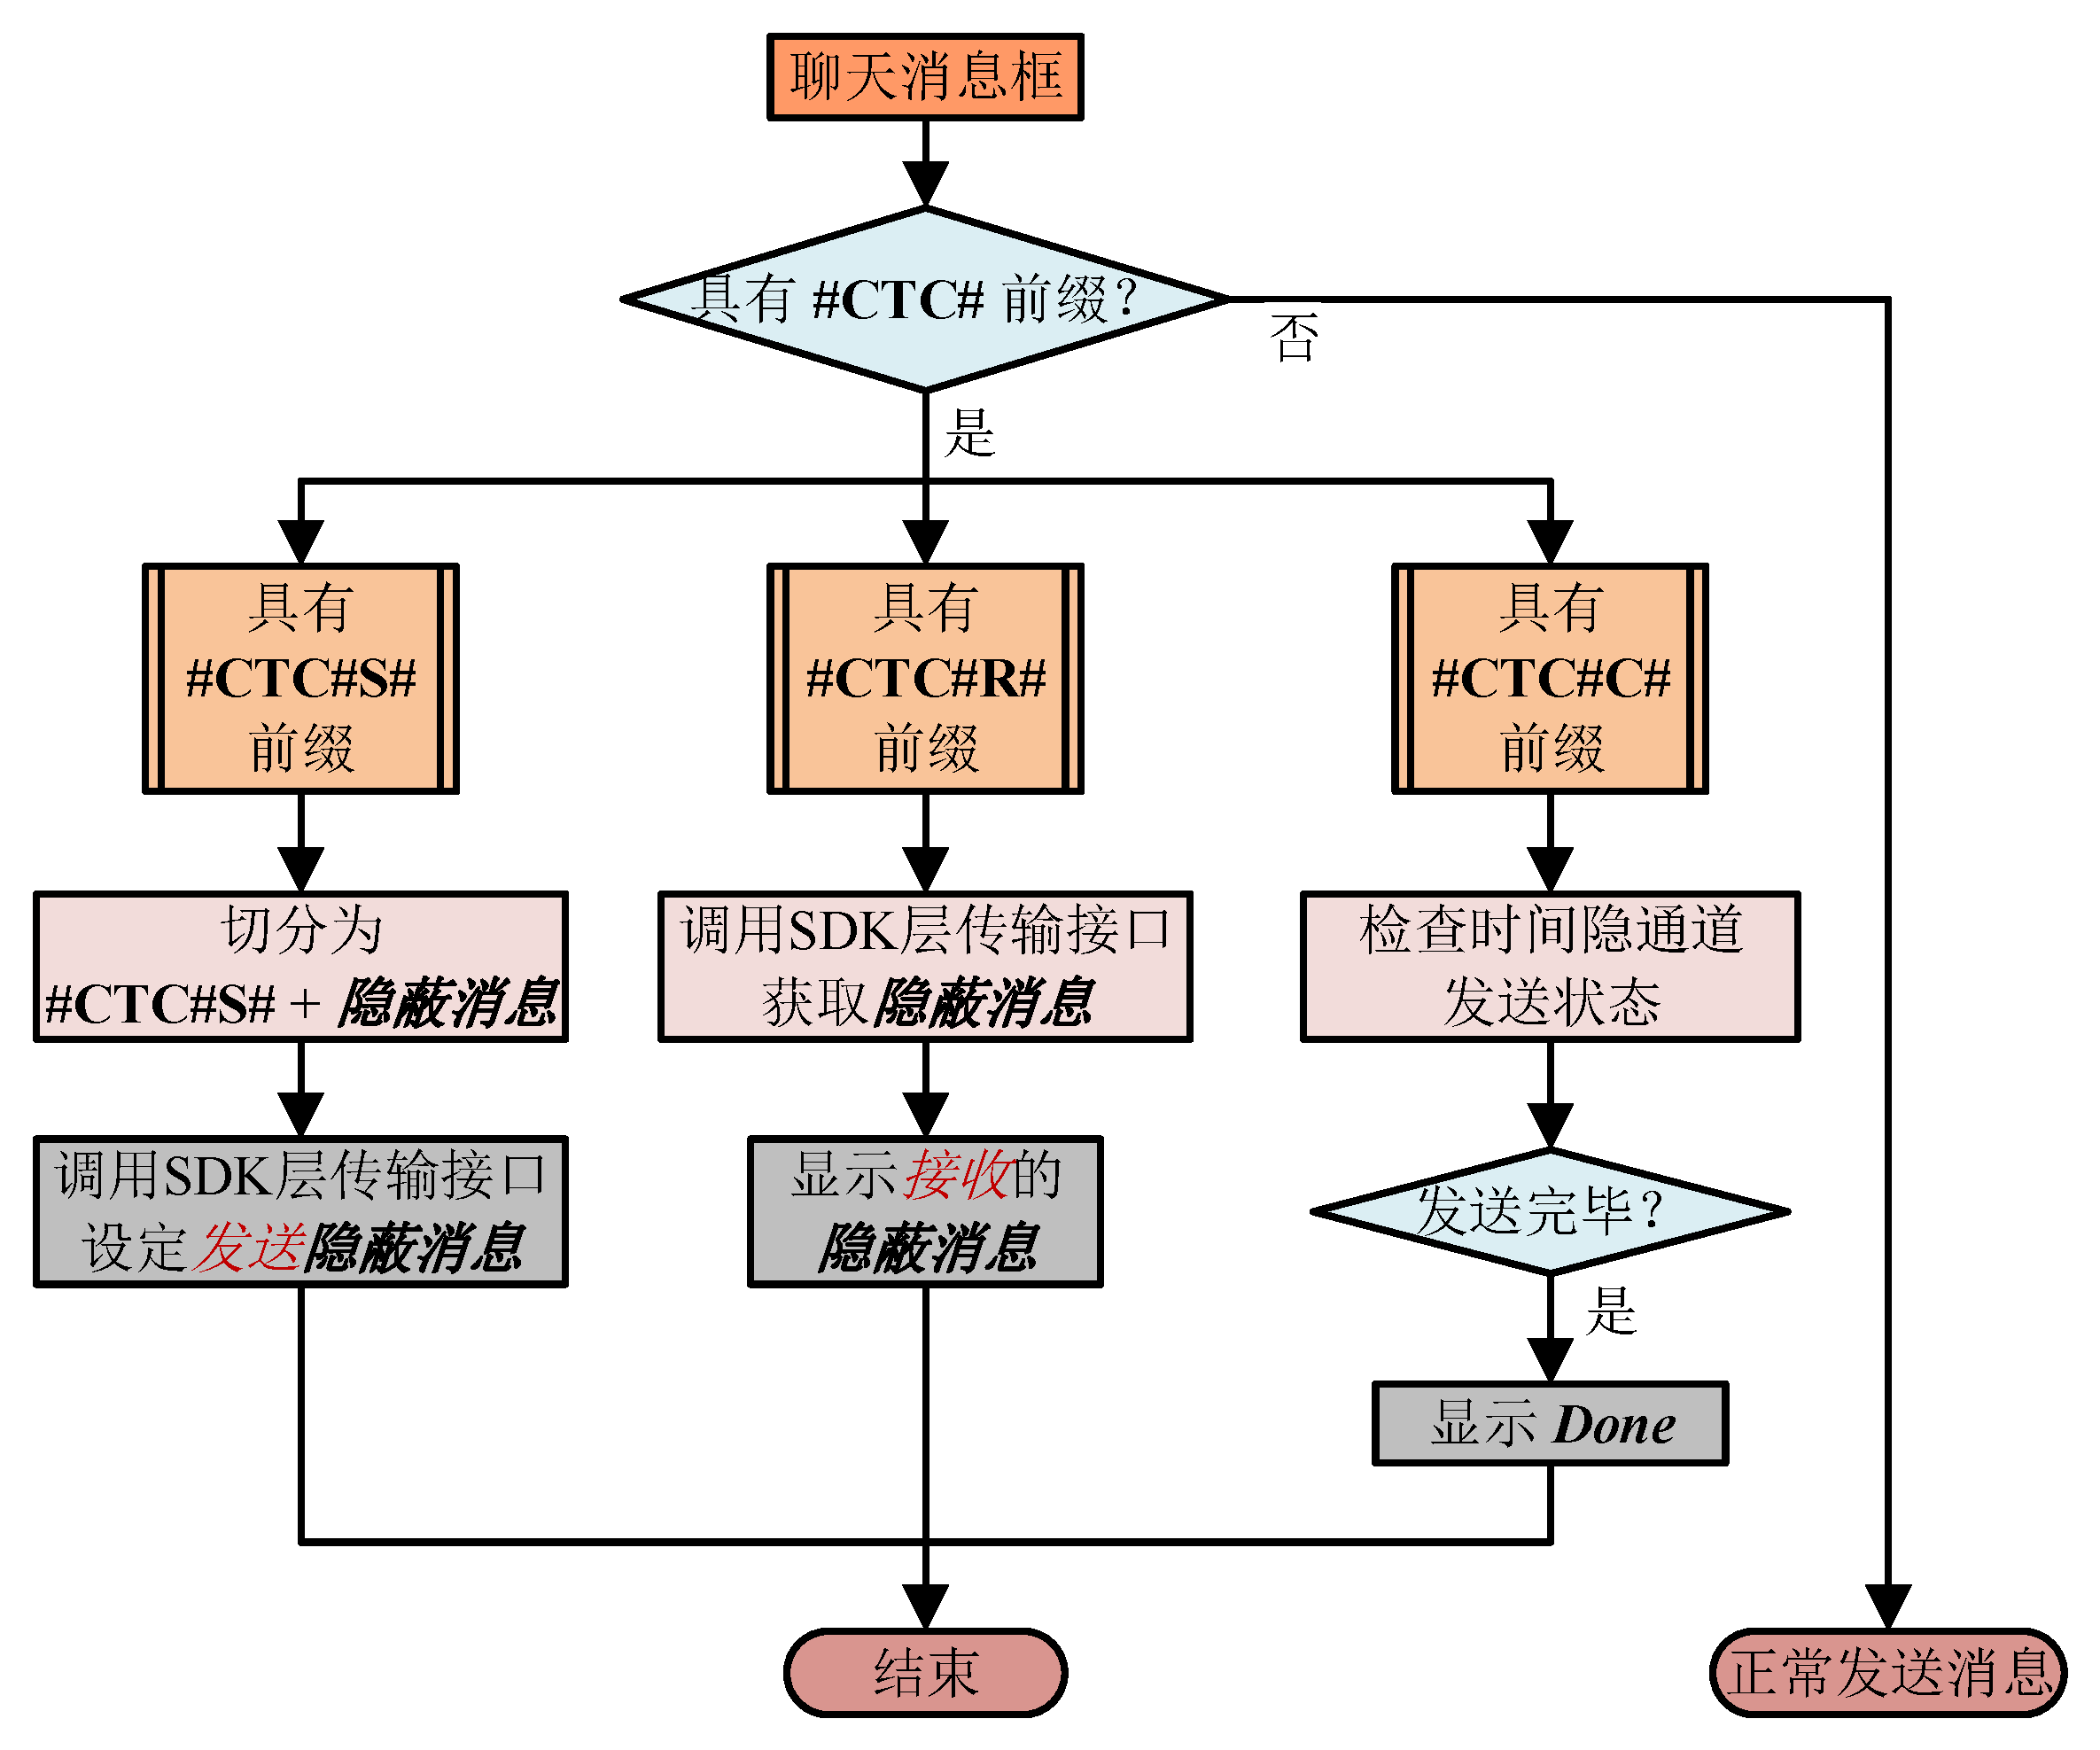
\includegraphics[width=0.85\textwidth]{chapters/chapter6/figures/ui-flow.pdf}
        \caption{用户界面的控制接口设计}
        \label{fig:6:ui-flow}
    \end{figure}
}

如图\nref{fig:6:ui-flow},在UI层为时间隐通道提供了三个控制接口,分别对应发送隐蔽消息、获取隐蔽消息及检查发送状态。三种接口均通过聊天界面输入框进行触发,前缀‘\#CTC\#S\#’对应发送隐蔽消息,前缀‘\#CTC\#R\#’对应获取隐蔽消息,前缀‘\#CTC\#C\#’对应检查发送状态。当触发隐蔽消息发送时,首先将输入内容进行切分,前缀‘\#CTC\#S\#’后的内容设定为隐蔽消息,调用SDK层的隐通道传输接口进行设定。当触发隐蔽消息接收时,调用SDK层的隐通道传输接口,获取当前已经接收的隐蔽消息,并在输入框中进行显示。当触发发送状态检查时,调用SDK层的隐通道传输接口,判断当前隐蔽消息是否传输完毕,如传输完毕则显示‘Done’确认。

\subsection{oRTP传输控制设计}
\label{chap:linphone:designation:ortp}

\insertFigure{
	\begin{figure}
		\centering
        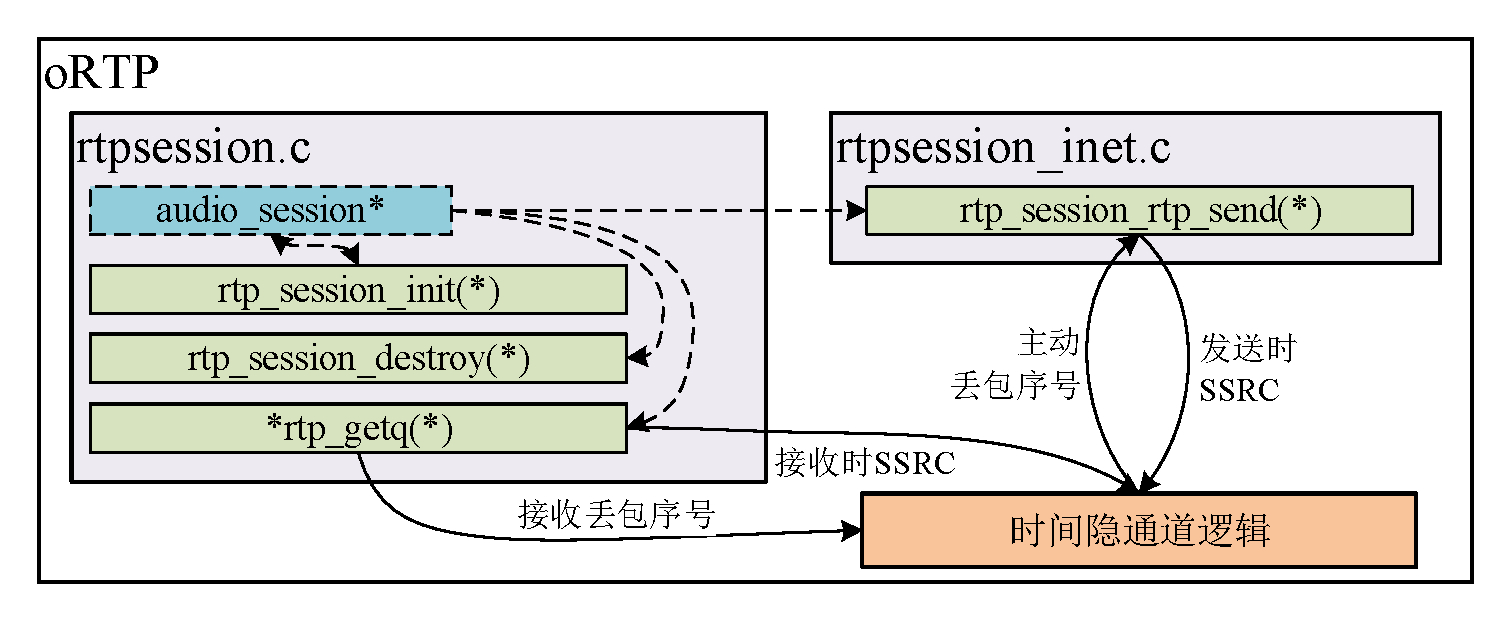
\includegraphics[width=0.85\textwidth]{chapters/chapter6/figures/ortp-flow.pdf}
        \caption{oRTP中时间隐通道的数据流}
        \label{fig:6:ortp-flow}
    \end{figure}
}

oRTP中添加的功能主要包含三部分,分别为语音数据流识别、接收丢包序号监听以及主动丢包控制。其中,语音数据流识别与接收丢包序号监听位于rtpsession.c文件中,接收丢包序号监听位于rtpsession\_inet.c文件中。语音数据流识别通过指针audio\_session记录语音会话的指针,当执行rtp\_session\_init初始化时进行赋值,通话结束后执行rtp\_session\_destroy时进行清理。接收丢包序号监听在rtp\_getq函数内部实现,根据audio\_session识别语音数据流后,由数据包接收队列中判断出未接收到的序号,并将结果传输到时间隐通道逻辑组件。接收丢包序号监听在rtp\_session\_rtp\_send函数内部实现,该函数将数据包由发送队列中取出后,交付网络组件进行传输,通过判断数据包序号是否为时间隐通道要丢弃的目标,执行传输或销毁操作。此外,在接收与发送过程中,将RTP包头中的SSRC字段反馈到时间隐通道逻辑组件,用于调制与解调中的随机化处理。

\subsection{消息传输机制设计}
\label{chap:linphone:designation:data}

\insertFigure{
	\begin{figure}
		\centering
        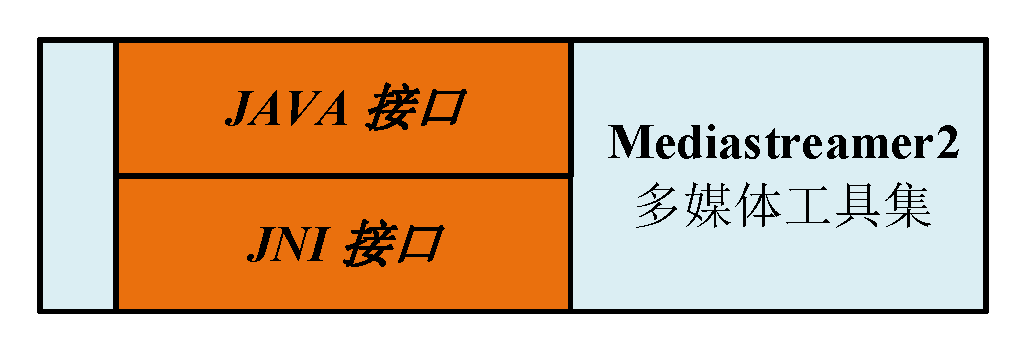
\includegraphics[width=0.5\textwidth]{chapters/chapter6/figures/data-flow.pdf}
        \caption{消息传输接口的结构构成}
        \label{fig:6:data-flow}
    \end{figure}
}

如图\nref{fig:6:data-flow},Mediastreamer2中时间隐通道的消息传输接口,主要由两部分组成。接口包含Linphone SDK提供给UI层的JAVA接口,以及面向oRTP层中时间隐通道逻辑组件的JNI调用。根据Linphone的软件设计架构,Linphone SDK与UI层通过接口进行数据传输,从而实现内存隔离及内部数据保护。因此,时间隐通道要完成UI层到oRTP层的交互,需要按照相同的模式添加各部分接口。在数据类型方面,需要由JNI函数实现JAVA数据类型与C数据类型转换,从而实现消息的正确传输。

\subsection{调制解调方法设计}
\label{chap:linphone:designation:modulation}

本文中提出了两种时间隐通道构建方法,二者均采用参数$L_{Codeword}$控制主动丢包密度,其主要区别为调制解调中消息与丢包序号的转换方法。在Linphone环境中验证时间隐通道构建方法,在网络稳定性与一致性方面与VoLTE存在差异,因此对调制解调方法进行简化处理。由于Linphone支持NAT转换,当通话稳定后,语音信道中的噪声干扰较少。因此,时间隐通道在通话开始,并传输200个数据包后才开始运作,按照语音数据包50\ packets/s的发送速率,200个数据包对应4s左右的通话时间。

\insertFigure{
	\begin{figure}
		\centering
        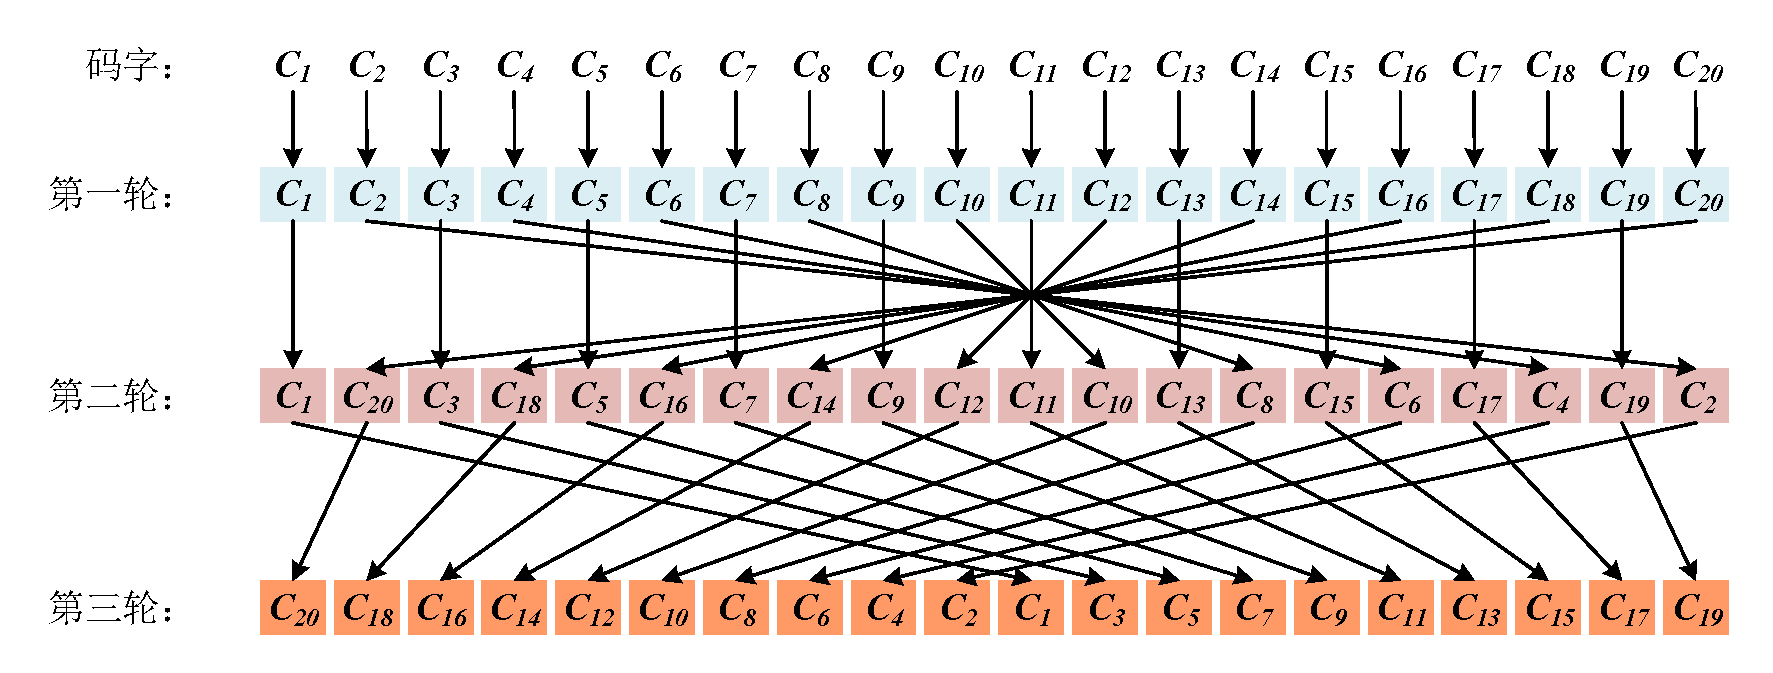
\includegraphics[width=0.95\textwidth]{chapters/chapter6/figures/codeword-cycle.pdf}
        \caption{时间隐通道中码字发送轮次及顺序}
        \label{fig:6:codeword-cycle}
    \end{figure}
}

如图\nref{fig:6:ortp-flow},RTP包头中的SSRC反馈到时间隐通道逻辑组件中,实现传输过程随机化。以SSRC作为随机数种子,每组迭代伪随机数生成器,计算其对应的偏移量。如图\nref{fig:6:codeword-cycle},每个码字都会被重复发送三次,每轮按照不同的顺序进行组织。时间隐通道接收方,将数据包序号转换为每组中的码字后,将三个轮次得到的结果取交集,从而去除网络噪声干扰。

\subsection{Linphone中时间隐通道工作流程}
\label{chap:linphone:designation:workflow}

\insertFigure{
	\begin{figure}
		\centering
        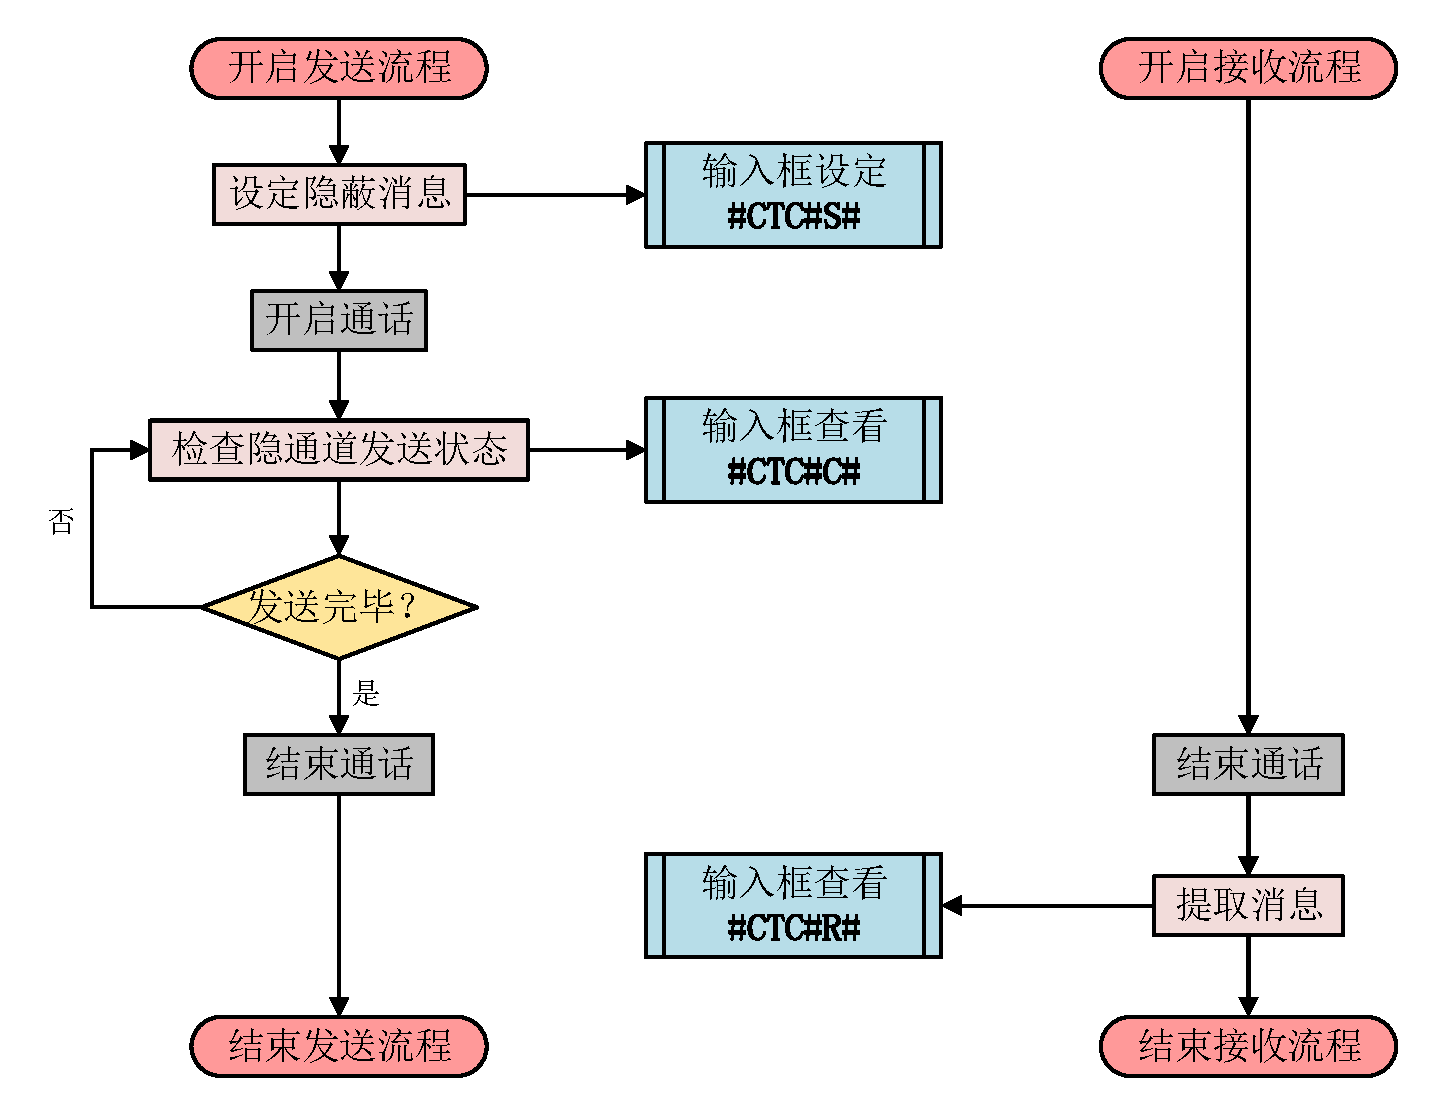
\includegraphics[width=0.7\textwidth]{chapters/chapter6/figures/call-ctc.pdf}
        \caption{Linphone通话与时间隐通道工作流程}
        \label{fig:6:call-ctc}
    \end{figure}
}

如图\nref{fig:6:call-ctc},时间隐通道的工作流程,与Linphone的通话过程密切相关。基于主动丢包的时间隐通道工作在双工状态,可以同时进行发送与接收,并且两个过程间无干扰。对于发送流程来说,首先要设置待发送的隐蔽消息,然后开启通话。当消息发送完毕,发送方查看状态确认后,即可关闭通话。接收流程通过监听数据包序号,在通话结束后还原隐蔽消息,隐通道接收方查看消息内容,接收流程完毕。在双工模式下,通话双方既是发送方又是接收方,具备信息交换能力。